\section{Coq による形式化}

本節では,3節で述べた \api についてどのように Coq で記述していくかについて説明する.
まず%% 名前,\conf,\conf 中の\free,
仮名関数およびその性質についての Coq での表現を述べる.
次に型付け規則を Coq で使いやすくための規則の具体化を説明し,最後に型システムの健全性の Coq での証明方針を述べる.
また,Coq による定義と証明の全文は GitHub リポジトリ\cite[api]{api}に公開している.
%% また,Coq のバージョンは 8.4pl4 を用いている.
%% 本研究では,アクターの振る舞いに関するこの3つの補題について,Coq を使って形式的な証明を与える.

%% \begin{itemize}
%% \item 振る舞いのインスタンス化について,そのアクターが仮の名前を持つか持たないかによって別個の定義にした
%% \item

%% \section{\conf}

%% \conf は \srcref{coq:conf} のように帰納的に定義した.各コンストラクタの対応関係は 表\ref{coq:conf_table} である.
%% 振る舞いのインスタンス化 $\instantiate{\tilde{u}}{\tilde{v}}{u_1}{z}{P}{\tilde{x}}{\tilde{y}}$ については $len(\tilde{x})$ が1の場合と2の場合で場合分けをしている.

%% \begin{figure}[tbph]
%%   \lstinputlisting[]{./src/config.v}
%%   \caption{\conf}
%%   \label{coq:conf}
%% \end{figure}

%% \begin{table}[tbph]
%%   \caption{\conf の対応関係}
%%   \begin{center}
%%     \begin{tabular}{|ll|}
%%       \hline
%%       $P$                    & {\tt config} \\ \hline
%%       $\nilconf$             & {\tt nil} \\
%%       $\actorconf{x}{y}{P}$  & {\tt create x y P} \\
%%       $\sendconf{x}{y}$      & {\tt send x y} \\
%%       $\restrictconf{x}{P}$  & {\tt restrict x P} \\
%%       $\composeconf{P1}{P2}$ & {\tt compose P1 P2} \\
%%       $\caseconf{x}{y_1 : P_1, ..., y_n : P_n}$ & {\tt caseof x [(y1, P1), ..., (yn, Pn)]} \\
%%       $\instantiate{\tilde{u}}{\tilde{v}}{u_1}{z}{P}{\tilde{x}}{\tilde{y}}$   & {\tt instantiate\_1 u v z p x y}, \\
%%                              & {\tt instantiate\_2 u1 u2 v z p x1 x2 y} \\
%%       \hline
%%     \end{tabular}
%%     \label{coq:conf_table}
%%   \end{center}
%% \end{table}


%% また,名前 $x$ は \conf $P$ 中に現れる\free である,という関係を \srcref{coq:free} のように帰納的に定義した.

%% \begin{figure}[tbph]
%%   \lstinputlisting{./src/free.v}
%%   \caption{\conf と\free の関係}
%%   \label{coq:free}
%% \end{figure}


\subsection{\tmp}

仮につけた名前から正規の名前を得る \tmp の Coq での定義について述べる.

\tmp $ f $ の型は $X \rightarrow X^* $ であり,定義域と値域の集合は $\bot$ と $\ast$ を除くと等しくなっている.
Coq による形式化では簡単にするためにその情報を捨て,任意の {\tt name} 型の値から任意の {\tt option star} 型への関数とした.
定義域の範囲に入っていない入力は {\tt None} を返すことを想定している.
また,ここで {\tt star} 型は {\tt name} 型に $\bot$ と $\ast$ という値を加えたような型である.

この変更により,以下の述語が必要となる.$f : X \rightarrow X^*$ ということを,$in\_range\_in\_domain(f)$ を満たすことで表している.

\begin{dfn}[$in\_domain$]
  名前 $x$ ,\tmp $f$ について,$x \in domain(f)$ を $in\_domain(f,x)$ で表す.ただし $domain(f)$ は $f$ の定義域である.
\end{dfn}

\begin{dfn}[$in\_range$]
  名前 $x$ ,\tmp $f$ について,$x \in range(f)$ を $in\_range(f,x)$ で表す.ただし $range(f)$ は $f$ の値域である.
\end{dfn}

\begin{dfn}[$in\_range\_in\_domain$]
  ある \tmp $f$ が,任意の名前 $x$ について $in\_range(f, x) \Rightarrow in\_domain(f, x)$ を満たすということを \\
  $in\_range\_in\_domain(f)$ で表す.
\end{dfn}

%% \begin{figure}[tbph]
%%   \lstinputlisting{./src/range_domain.v}
%%   \caption{述語 $in\_domain, in\_range, in\_range\_in\_domain$}
%%   \label{coq:range_domain}
%% \end{figure}

また,2つの \tmp の定義域が重なっていないことを表す述語 $fun\_exclusive$ を定義する.

\begin{dfn}[$fun\_exclusive$]
  2つの \tmp $f : X \rightarrow X^*, g : Y \rightarrow Y^*$ について,$X \cap Y = \emptyset$ であるという述語を $fun\_exclusive$ と定義する.
%% 述語をある名前 $x$ が $f$ の定義域の要素であるならば $x$ は $g$ の定義域の要素ではない,かつ,$x$ が $g$ の定義域の要素であるならば $x$ は $f$ の定義域のではない,
\end{dfn}

%% これは述語 $in\_domain$ を使って \srcref{coq:fun_exclusive} のように定義できる.

%% \begin{figure}[tbph]
%%   \lstinputlisting{./src/fun_exclusive.v}
%%   \caption{$fun\_exclusive$}
%%   \label{coq:fun_exclusive}
%% \end{figure}

  %% $ \bot, \ast \notin {\cal N}, X \subset {\cal N}, X^* = X \cup \{\bot,\ast\} $
  %% \begin{table}[htb]
  %%   \begin{tabular}{ll}
  %%     $ f(x) $ & if $ x $ is a regular actor name \\
  %%     $ f(x) = \ast $ & if $ x $ is the temporary name \\
  %%     \ & of an actor with a private name \\
  %%     $ f(x) = y \notin \{\bot,\ast\} $ & means that actor $ y $ has assumed \\
  %%     \ & the temporary name $ x $
  %%   \end{tabular}
  %% \end{table}
  %% and $ f^* : X^* \rightarrow X^* $ as $ f^*(x) = f(x) \  for \ x \in X $ and $ f^*(\bot) = f^*(\ast) = \bot $

\subsubsection{\tmp の構築}

\tmp は $ch$ 関数,\tmp の合成,\tmp の値域の制限,のいずれかで作ることができる.
ここで,$ch$ 関数が使われている型付け規則は \textsc{Act} のみであるが,この中で使われている $ch$ 関数は入力の要素数が0個,1個,2個のものしかない.
よって,$ch$ 関数はこの3パターンに限定でき,それぞれ $ch_0, ch_1, ch_2$ と書くこととする.
また,\tmp の値域の制限を行う二項演算子 $(|)$ が現れるのは \textsc{Res} のみで,かつそれはもとの仮名関数の値域からあるひとつの要素を取り去るものとしてしか使われていない.
後の証明を簡単にするために,この演算子を,制限後の集合ではなく値域から取り去る要素を右手にとるものとして定義する.
ただし,この演算子はもとの演算子 $(|)$ とは定義が異なるため,混乱を避けるために別の記号 $(\setminus)$ を用いることにする.

\begin{dfn}[\tmp の値域の制限]
  $f : \rho \rightarrow \rho^*, x \in \rho$ である $f, x$ に対して値域の制限を表す二項演算子 $f \setminus x : \rho - \{x\} \rightarrow (\rho - \{x\})^*$ を以下のように定義する. \\
\begin{adjustvboxheight}
  \[ (f \setminus x)(y) = \begin{cases}
    \ast & f(y) = x \mbox{のとき} \\
    f(y) & \mbox{その他}
  \end{cases} \]
  \vspace{1pt}
\end{adjustvboxheight}
\end{dfn}


また,$ch_0, ch_1, ch_2, \oplus, \setminus$ について仮名関数の性質を満たすことを証明した.
その際,$ch_2$ は引数である2つの名前が異なることを,$\oplus$ は $in\_domain\_in\_range, fun\_exclusive$ が成り立つという前提を加えている.

%% 以上の5つを \srcref{tmp_fun} と定義した.


%% %% 型付け規則 \textsc{Act} を分割した \textsc{Act-empty}, \textsc{Act-x}, \textsc{Act-z}, \textsc{Act-xz} のみであるが,これらの規則内の

%% \begin{figure}[tbph]
%%   \lstinputlisting{./src/tmp_fun.v}
%%   \caption{\tmp の構築}
%%   \label{tmp_fun}
%% \end{figure}

%% \subsection{\tmp の性質}

%% \tmp を構築するものは,5種しかなかったが,これら全てにおいて\tmp の性質を満たす.\tmp の性質は Coq では \srcref{coq:tmp_prop} と定義した.

%% \begin{figure}[tbph]
%%   \lstinputlisting{./src/tmp_prop.v}
%%   \caption{\tmp の性質}
%%   \label{coq:tmp_prop}
%% \end{figure}

%% それぞれの要素を用いて構築された\tmp について,それが\tmp の性質を満たすという補題を証明する必要がある.

%% \begin{lem}[\tmp の性質($ch_0$)]
%%   \label{lemma:ch_0_prop}
%%   $ch_0$ は \tmp の性質を満たす.
%% \end{lem}

%% \begin{lem}[\tmp の性質($ch_1$)]
%%   \label{lemma:ch_1_prop}
%%   $ch_1$ は \tmp の性質を満たす.
%% \end{lem}

%% \begin{lem}[\tmp の性質($ch_2$)]
%%   \label{lemma:ch_2_prop}
%%   $ch_2$ は,2つの入力 $x, y$ について $x \neq y$ であるならば,\tmp の性質を満たす.
%% \end{lem}

%% \begin{lem}[\tmp の性質($fun\_plus$)]
%%   \label{lemma:fun_plus_prop}
%%   \tmp $f, g$ が \tmp の性質,$range\_domain$,$fun\_exclusive$ を満たすならば,$fun\_plus(f, g)$ は \tmp の性質を満たす.
%% \end{lem}

%% \begin{lem}[\tmp の性質($fun\_remove$)]
%%   \label{lemma:fun_remove_prop}
%%   \tmp $f$ が \tmp の性質満たすならば,任意の名前 $x$ について $fun\_remove(f, x)$ は \tmp の性質を満たす.
%% \end{lem}

%% これらの補題は,Coq では\srcref{coq:fun_prop} のように定義した.

%% \begin{figure}[htbp]
%%   \lstinputlisting{./src/fun_prop.v}
%%   \caption{\tmp の性質の補題}
%%   \label{coq:fun_prop}
%% \end{figure}


%% 以下の補題は \tmp の Coq での定義に,定義域と値域の情報が入っていないことによる補題(元の定義では自明)


%% また,二つの\tmp $f_1, f_2$ が互換性を持つという述語,及び\tmp $f_1, f_2, ..., f_n$ が相互に互換性を持つという述語を,\srcref{coq:compatible} と定義した.

%% \begin{figure}[tbph]
%%   \lstinputlisting{./src/compatible.v}
%%   \caption{互換性}
%%   \label{coq:compatible}
%% \end{figure}


\subsection{型付け規則}

%% 本節では,\api の型付け規則を Coq で定義する.

\api の型付け規則には,Coq 上で定義しにくい,またはそのままでは証明を進めにくいものがある.実際に Coq で型付け規則を定義する前に,型付け規則を再定義する.

\subsubsection{\textsc{Act} 規則の分割}

型付け規則 \textsc{Act} はアクターが作られる際に考えられるパターンを複数まとめたものであり,このままの定義を用いると証明が煩雑になってしまう.
これは,\textsc{Act} に関する証明を行う際に,$ch$ 関数の定義にともなって \textsc{Act} に現れる $\rho$ の要素数で場合分けをすることになるが,その都度考えられない場合が現れ,その場合は矛盾を証明する,ということをしなければならないためである.
また,Coq では任意の要素数を持つ集合を扱うような証明は煩雑になってしまいやすい.
そこで,事前に $\rho$ の要素数によって場合分けを行い,\textsc{Act} を分割しておくことを考える.
$\rho$ の場合分けを行うと,以下のように4つに分けられることがわかる.

\begin{enumerate}
  \item 要素数が0のとき \\
    $\rho - \{x\} = \hat{z}$ から,$\hat{z} = \emptyset, f = ch_0$ である.
  \item 要素数が1のとき
    \begin{enumerate}
      \item $x \in \rho$ のとき \\
        $\rho - \{x\} = \hat{z}$ で $len(\rho) = 1$ なので,$\hat{z} = \emptyset, f = ch_1(x)$ である.
      \item $x \notin \rho$ のとき \\
        $\rho - \{x\} = \hat{z}$ であるから,$len(\hat{z}) = 1$ である.$\hat{z} = \{z\}$ とすると,$f = ch_1(z)$ である.
    \end{enumerate}
  \item 要素数が2のとき \\
    $\rho - \{x\} = \hat{z}$ であり,$\hat{z}$ は要素数が $0$ または $1$ なので,$x \in \rho$ である.$\hat{z} = \{z\}$ とすると,$f = ch_2(x,z)$ である.
  \item 要素数が3以上のとき \\
    $3 \leq len(\rho)$ のとき,$\hat{z} (= \rho - \{x\})$ は要素数が2以上である.これは $\hat{z}$ の定義と矛盾する.よって要素数が3以上であることはない.
\end{enumerate}


この場合分けをもとに,\textsc{Act} を4つに分割すると,\srcref{coq:act} のような定義にできる.

\begin{figure}[t]
  \infrule[Act-empty]{
    \typing{\emptyset}{ch_0}{P}
  }{
    \typing{\{x\}}{ch_1(x)}{x(y).P}
  }
  \vspace{14pt}
  \infrule[Act-x]{
    \typing{\{x\}}{ch_1(x)}{P}
    \andalso x \neq y
  }{
    \typing{\{x\}}{ch_1(x)}{x(y).P}
  }
  \vspace{14pt}
  \infrule[Act-z]{
    \typing{\{z\}}{ch_1(z)}{P}
    \andalso x \neq z
    \andalso y \neq z
  }{
    \typing{\{x, z\}}{ch_2(x, z)}{x(y).P}
  }
  \vspace{14pt}
  \infrule[Act-xz]{
    \typing{\{x, z\}}{ch_2(x, z)}{P}
    \andalso x \neq z
    \andalso x \neq y
    \andalso y \neq z
  }{
    \typing{\{x, z\}}{ch_2(x, z)}{x(y).P}
  }

  \caption{型付け規則\textsc{Act} の分割}
  \label{coq:act}
\end{figure}


\subsubsection{\textsc{Case} 規則の分割}

型付け規則 \textsc{Case} は,前提の数がパターンの数に依存して変動するので,Coq で定義しにくい.よって \srcref{api:case_split} のように \textsc{Case} をパターンが $0$ 個の場合と $i + 1$ に分割し,帰納的に定義する.これで,\textsc{Case} 規則の前提の数はパターンの数によらず一定となる.


\begin{figure}[t]
  \infrule[Case-nil]{
  }{
    \typing{\emptyset}{\{\}}{\caseconf{x}{}}
  }
  \vspace{14pt}
  \infrule[Case-cons]{
    \typing{\rho}{f}{\caseconf{x}{y_1 : P_1, ... , y_i : P_i}}
    \\
    \andalso \typing{\rho'}{f'}{P}
    \andalso compatible(f, f')
  }{
    \typing{\rho \cup \rho'}{f \oplus f'}{\caseconf{x}{y : P, y_1 : P_1, ... , y_i : P_i}}
  }

  \caption{型付け規則\textsc{Case} の分割}
  \label{api:case_split}
\end{figure}


また,この定義によって作られる型付け
\begin{center}
  $\typing{(...((\rho_1 \cup \rho_2) \cup \rho_3)... \cup \rho_n) \cup \rho}{(...((f_1 \oplus f_2) \oplus f_3)... \oplus f_n) \oplus f}{\caseconf{x}{y : P, y_1 : P_1, ..., y_n : P_n}}$
\end{center}
において,元の定義では $f, f_1, f_2, ..., f_n$ が相互に互換性を持つことを条件としているが,
$f, f_1, ..., f_n$ が相互に互換性を持つことは自明ではない.よって以下の補題が必要となる.

\begin{lem}
  仮名関数 $f, f_1, f_2$ について,$f$ と $f_1 \oplus f_2$ が互換性を持ち,$f_1$ と $f_2$ もまた互換性を持つとき,$f, f_1, f_2$ は相互に互換性を持つ.
  \label{lem:compatible}
\end{lem}

この補題の Coq による証明は \texttt{Fun} モジュールの \texttt{fun\_plus\_compatible} という名前にあるが,以下にその概略を示す.

まず $f$ と $f_1$ が $\oplus$ について可換であること, $f$ と $f_2$ が $\oplus$ について可換であることを,$f$ と $f_1 \oplus f_2$ が互換性を持ち $f_1$ と $f_2$ もまた互換性を持つという仮定から示す.このことから,$f$,$f_1$,$f_2$ が相互に可換になることがわかる.
次に,$f$,$f_1$,$f_2$ の任意の組み合わせの合成が\tmp の性質を満たすことを証明する.まずは $f$ と $f_1$ の合成が仮名関数の性質を満たすことを証明する.
$f$ と $f_1 \oplus f_2$ が互換性を持つという仮定から,$f \oplus (f_1 \oplus f_2)$ が仮名関数の性質を満たす.また仮名関数の合成は結合律が成り立つので $(f \oplus f_1) \oplus f_2$ も仮名関数の性質を満たす.
合成が仮名関数の性質を満たしているならば合成の左手は仮名関数の性質を満たす,という性質 (\texttt{fun\_prop\_plus\_fst} という名前で証明済み) を,先に証明した $(f \oplus f_1) \oplus f_2$ も仮名関数の性質を満たすということに使うと,$f \oplus f_1$ が仮名関数の性質を満たすということを導ける.
$f$ と $f_2$ についても同様である.また,$f_1$ と $f_2$ については仮定から明らかである.
以上から,$f$,$f_1$,$f_2$ の任意の組み合わせの合成が\tmp の性質を満たすことがわかったので,$f$,$f_1$,$f_2$ が相互に可換になることと合わせると,$f$,$f_1$,$f_2$ は相互に互換性を持つことがわかる.

この補題によって,$f, f_1, ... , f_n$ が相互に互換性を持つことが帰納的に保証される.%% この補題は Coq では \srcref{coq:fun_plus_compatible} と定義できる.

%% \begin{figure}[tbph]
%%   \lstinputlisting{./src/fun_plus_compatible.v}
%%   \caption{補題 \ref{lem:compatible} の Coq での定義}
%%   \label{coq:fun_plus_compatible}
%% \end{figure}


\subsubsection{\textsc{Res} 規則}

\tmp の値域の制限を行う二項演算子の定義を変更したことに合わせて,型付け規則 \textsc{Res} は \srcref{api:res_rule} のようになる.

\begin{figure}[t]
  \infrule[Res]{
    \typing{\rho}{f}{P}
  }{
    \typing{\rho - \{x\}}{f \setminus x}{\restrictconf{x}{P}}
  }
  \caption{型付け規則 \textsc{Res}}
  \label{api:res_rule}
\end{figure}

\subsubsection{\textsc{Inst} 規則の分割}

Coq による定義では振る舞いの雛形からアクターを作る\conf $\behaviorconf{\tilde{x}}{\tilde{y}} (B \defeq \behaviortemplate{\tilde{u}}{\tilde{v}}{u_1}{z}{P})$ を,$\tilde{u}$ の要素数が1である場合と2である場合で二つに分割している.
よって型付け規則も二つに分割する必要があり,\srcref{api:inst_rule} のようになる.
ただし,ここでは $B$ を使う代わりに $B$ の展開後の項を用いている.

\begin{figure}[t]
  \infrule[Inst-1]{
    \typing{\{u\}}{ch_1(u)}{\actorconf{u}{z}{P}}
  }{
    \typing{\{x\}}{ch_1(x)}{\instantiate{\tuple{u}}{\tilde{v}}{u}{z}{P}{\tuple{x}}{\tilde{y}}}
  }
  \vspace{14pt}
  \infrule[Inst-2]{
    \typing{\{u_1,u_2\}}{ch_2(u_1,u_2)}{\actorconf{u_1}{z}{P}}
    \andalso x_1 \neq x_2
  }{
    \typing{\{x_1, x_2\}}{ch_2(x_1, x_2)}{\\ \ \ \ \ \ \ \ \ \instantiate{\tuple{u_1,u_2}}{\tilde{y}}{u_1}{z}{P}{\tuple{x_1,x_2}}{\tilde{y}}}
  }
  \caption{型付け規則 \textsc{Inst} の分割}
  \label{api:inst_rule}
\end{figure}


%% \subsection{型付け規則の Coq での定義}

%% 分割後を含めた型付け規則全体の Coq 上での定義を \srcref{typing} に示す.型付け規則を素直に表現することで定義することができた.

%% \begin{figure}[tbph]
%%   \ContinuedFloat
%%   \lstinputlisting[basicstyle=\small]{./src/typing.v}
%%   \caption{型付け規則}
%%   \label{typing}
%% \end{figure}

\subsection{健全性の証明}


最後に健全性の証明を行うが,以下の3つの補題を証明しておくと,健全性の証明を行いやすいので証明しておく.対応する Coq による証明は,\texttt{Typing.v} ファイルの \texttt{typing\_in\_range\_in\_domain},\texttt{typing\_in\_domain\_1} および \texttt{typing\_in\_domain\_2},\texttt{Soundness.v} ファイルの \texttt{typing\_fun\_exclusive} にある.
%% \begin{figure}[tbph]
%%   \lstinputlisting{./src/fun_ext.v}
%%   \caption{関数の外延的同値}
%%   \label{coq:fun_ext}
%% \end{figure}


\begin{lem}[定義域と値域の一致]
  \label{lemma:typing_range_domain}
  $\typing{\rho}{f}{P}$ ならば,$in\_range\_in\_domain(f)$ が成り立つ.
\end{lem}

\begin{lem}[\tmp の定義域と\recep の一致]
  \label{lemma:typing_recep_domain}
  $\typing{\rho}{f}{P}$ ならば,任意の名前 $ x $ について $in\_domain(f, x) $ であるとき,かつそのときに限り,$ x \in \rho $ が成り立つ.
\end{lem}

\begin{lem}[$fun\_exclusive$ における集合の一致]
  \label{lemma:typing_fun_exclusive}
  $\typing{\rho_1}{f_1}{P_1}$ かつ $\typing{\rho_2}{f_2}{P_2}$ であり $ \rho_1 \cap \rho_2 \neq \emptyset $ ならば,$fun\_exclusive(f_1, f_2)$ を満たす.
\end{lem}

健全性は,以上の公理と補題を利用して,型付け規則の構造に関する帰納法で証明できる.対応する Coq の証明は \texttt{Soundness.v} ファイルの \texttt{Soundness} にある.

%% これらの補題は,Coq では \srcref{coq:lemma} のように定義した.


%% \begin{figure}[tbph]
%%   \lstinputlisting{./src/lemma.v}
%%   \caption{健全性の証明に必要となる補題}
%%   \label{coq:lemma}
%% \end{figure}

%% \subsection{Coq での定義と証明}

%% \api の健全性の定理は,\srcref{soundness} のように定義した.

%% \begin{figure}[tbph]
%%   \lstinputlisting{./src/soundness.v}
%%   \caption{健全性}
%%   \label{soundness}
%% \end{figure}

%% 証明の全文は付録Aに示した.ここでは\api の健全性の3つの要素である \recep の健全性,仮名の取り方についての健全性,型付けの一意性のそれぞれについて証明の方針について示す.

%% \subsubsection{\recep の健全性}

%% \recep の健全性は,次の方針で証明できる.

%% \begin{proof}
%%   型付けの構造に関する帰納法で証明する.

%%   \begin{enumerate}
%%     \item[(\textsc{Nil})]
%%       \recep は空集合なので明らか.
%%     \item[(\textsc{Msg})]
%%       \textsc{Nil} と同様に明らか.
%%     \item[(\textsc{Act-empty})]
%%       $\typing{\{x\}}{ch_1(x)}{\actorconf{x}{y}{P}}$ で,$x$ は $\actorconf{x}{y}{P}$ の\free であるので,命題を満たす.
%%     \item[(\textsc{Act-x})]
%%       \textsc{Act-empty} と同様に命題を満たす.
%%     \item[(\textsc{Act-z})]
%%       帰納法の仮定から,$z$ は $P$ の\free であり,$y \neq z$ という条件から,$z$ は $\actorconf{x}{y}{P}$ 中の\free である.
%%       また,$x$ も $\actorconf{x}{y}{P}$ 中の\free であるので,命題を満たす.
%%     \item[(\textsc{Act-xz})]
%%       \textsc{Act-z} と同様に命題を満たす.
%%     \item[(\textsc{Case-nil})]
%%       \textsc{Nil} と同様に明らか.
%%     \item[(\textsc{Case-cons})]
%%       帰納法の仮定から $\rho$ のすべての要素は $\caseconf{x}{y_1 : P_1, ..., y_i : P_i}$ 中の\free であり,$\rho'$ のすべての要素は $P$ 中の\free である.
%%       $\rho$ のすべての要素および $\rho'$ のすべての要素は,$\caseconf{x}{y : P, y_1 : P_1, ..., y_i : P_i}$ の\free であるので,$\rho \cup \rho'$ についてもこれを満たす.
%%     \item[(\textsc{Comp})]
%%       帰納法の仮定から,$\rho_1$ のすべての要素は $P_1$ の\free であり,$\rho_2$ のすべての要素は $P_2$ の\free である.
%%       よって $\rho_1 \cup \rho_2$ のすべての要素は $\composeconf{P_1}{P_2}$ の\free である.
%%     \item[(\textsc{Res})]
%%       帰納法の仮定から,$\rho$ のすべての要素は $P$ 中の\free である.
%%       $\restrictconf{x}{P}$ によって $x$ は\free ではなくなるが,$x$ は $\rho - \{x\}$ の要素ではないため,命題を満たす.
%%     \item[(\textsc{Inst-1})]
%%       $\typing{\{x\}}{ch(x)}{\instantiate{\tuple{u}}{\tilde{v}}{u}{z}{P}{\tuple{x}}{\tilde{y}}}$ で,$x$ は
%%       $\instantiate{\tuple{u}}{\tilde{v}}{u}{z}{P}{\tuple{x}}{\tilde{y}}$ の\free であるので,命題を満たす.
%%     \item[(\textsc{Inst-2})]
%%       $\typing{\{x_1,x_2\}}{ch_2(x_1,x_2)}{\instantiate{\tuple{u_1,u_2}}{\tilde{v}}{u_1}{z}{P}{\tuple{x_1,x_2}}{\tilde{y}}}$ で,$x_1,x_2$ は \\
%%       $\instantiate{\tuple{u_1,u_2}}{\tilde{v}}{u_1}{z}{P}{\tuple{x_1,x_2}}{\tilde{y}}$ の\free であるので,命題を満たす.
%%   \end{enumerate}
%% \end{proof}

%% \subsubsection{仮名の取り方の健全性}

%% 仮名の取り方の健全性は以下の方針で証明できる.

%% \begin{proof}
%%   型付けの構造に関する帰納法で証明する.

%%   \begin{enumerate}
%%     \item[(\textsc{Nil})]
%%       \lemmaref{lemma:ch_0_prop} より明らか.
%%     \item[(\textsc{Msg})]
%%       \textsc{Nil} と同様に明らか.
%%     \item[(\textsc{Act-empty})]
%%       \lemmaref{lemma:ch_1_prop} より明らか.
%%     \item[(\textsc{Act-x})]
%%       \lemmaref{lemma:ch_1_prop} より明らか.
%%     \item[(\textsc{Act-z})]
%%       \lemmaref{lemma:ch_2_prop} より明らか.
%%     \item[(\textsc{Act-xz})]
%%       \lemmaref{lemma:ch_2_prop} より明らか.
%%     \item[(\textsc{Case-nil})]
%%       \textsc{Nil} と同様に明らか.
%%     \item[(\textsc{Case-cons})]
%%       互換性の定義より明らか.
%%     \item[(\textsc{Comp})]
%%       \lemmaref{lemma:fun_plus_prop} ,\lemmaref{lemma:typing_range_domain} ,\lemmaref{lemma:typing_fun_exclusive} を使って証明できる.
%%     \item[(\textsc{Res})]
%%       \lemmaref{lemma:fun_remove_prop} より明らか.
%%     \item[(\textsc{Inst-1})]
%%       \lemmaref{lemma:ch_1_prop} より明らか.
%%     \item[(\textsc{Inst-2})]
%%       \lemmaref{lemma:ch_2_prop} より明らか.
%%   \end{enumerate}
%% \end{proof}

%% \subsubsection{型付けの一意性}

%% 型付けの一意性は以下の方針で証明できる.

%% \begin{proof}
%%   型付けの構造に関する帰納法で証明する.

%%   \begin{enumerate}
%%     \item[(\textsc{Nil})]
%%       $\nilconf$ の型付け規則は \textsc{Nil} 規則のみで,さらに\recep は空集合,\tmp は空関数なので,命題を満たす.
%%     \item[(\textsc{Msg})]
%%       $\sendconf{x}{y}$ ($x, y$ は任意) の型付け規則は \textsc{Msg} のみで,さらに\recep は空集合,\tmp は空関数なので,命題を満たす.
%%     \item[(\textsc{Act-empty})]
%%       この型付け規則の前提は $\typing{\emptyset}{ch_0}{P}$ であり,帰納法の仮定から,この $P$ の型付けは唯一である.
%%       $\typing{\{x\}}{ch_1(x)}{\actorconf{x}{y}{P}}$ となる型付け規則は \textsc{Act-empty}, \textsc{Act-x} の2種類あるが,$\typing{\emptyset}{\{\}}{P}$ から構築できるのは \textsc{Act-empty} のみであり,かつ\recep と\tmp は $x$ で構築されている.よって命題を満たす.
%%     \item[(\textsc{Act-x})]
%%       この型付け規則の前提は $\typing{\{x\}}{ch_1{x}}{P}$ であり,帰納法の仮定から,この $P$ の型付けは唯一である.
%%       $\typing{\{x\}}{ch_1(x)}{\actorconf{x}{y}{P}}$ となる型付け規則は \textsc{Act-empty}, \textsc{Act-x} の2種類あるが,$\typing{\{x\}}{ch_1(x)}{P}$ から構築できるのは \textsc{Act-x} のみであり,かつ\recep と\tmp は $x$ で構築されている.よって命題を満たす.
%%     \item[(\textsc{Act-z})]
%%       この型付け規則の前提は $\typing{\{z\}}{ch_1(z)}{P}$ であり,帰納法の仮定から,この $P$ の型付けは唯一である.
%%       $\typing{\{x,z\}}{ch_2(x,z)}{\actorconf{x}{y}{P}}$ (ただし $x \neq z$) となる型付け規則は \textsc{Act-z}, \textsc{Act-xz} の2種類あるが,$\typing{\{z\}}{ch_1(z)}{P}$ から構築できるのは \textsc{Act-z} のみであり,かつ\recep と\tmp は $x,z$ で構築されている.よって命題を満たす.
%%     \item[(\textsc{Act-xz})]
%%       この型付け規則の前提は $\typing{\{x,z\}}{ch_2(x,z)}{P}$ (ただし $x \neq z$) であり,帰納法の仮定から,この $P$ の型付けは唯一である.
%%       $\typing{\{x,z\}}{ch_2(x,z)}{\actorconf{x}{y}{P}}$ となる型付け規則は \textsc{Act-z}, \textsc{Act-xz} の2種類あるが,$\typing{\{x,z\}}{ch_2(x,z)}{P}$ から構築できるのは \textsc{Act-xz} のみであり,かつ\recep と\tmp は $x,z$ で構築されている.よって命題を満たす.
%%     \item[(\textsc{Case-nil})]
%%       $\caseconf{x}{}$ ($x$ は任意) の型付け規則は \textsc{Case-nil} のみで,さらに\recep は空集合,\tmp は空関数なので,命題を満たす.
%%     \item[(\textsc{Case-cons})]
%%       この型付け規則の前提は $\typing{\rho}{f}{\caseconf{x}{y_1 : P_1, ... , y_i : P_i}}$ および $\typing{\rho'}{f'}{P}$ であり,帰納法の仮定からこれらの型付けは一意である.
%%       $\typing{\rho \cup \rho'}{f \oplus f'}{\caseconf{x}{y : P, y_1 : P_1, ... , y_i : P_i}}$ となる型付け規則は \textsc{Case-cons} のみであり,かつ\recep は $\rho, \rho'$ ,\tmp は $f,f'$ で構築されている.よって命題を満たす.
%%     \item[(\textsc{Comp})]
%%       この型付け規則の前提は $\typing{\rho_1}{f_1}{P_1}$ および $\typing{\rho_2}{f_2}{P_2}$ であり,帰納法の仮定からこれらの型付けは一意である.
%%       $\typing{\rho_1 \cup \rho_2}{f_1 \oplus f_2}{P_1 \setminus P_2}$ となる型付け規則は \textsc{Comp} のみであり,かつ\recep は $\rho_1, \rho_2$ ,\tmp は $f_1,f_2$ で構築されている.よって命題を満たす.
%%     \item[(\textsc{Res})]
%%       この型付け規則の前提は $\typing{\rho}{f}{P}$ ,帰納法の仮定からこの型付けは一意である.
%%       $\typing{\rho - \{x\}}{f \setminus x}{(\nu x)P}$ となる型付け規則は \textsc{Res} のみであり,かつ\recep と\tmp は共に $\rho, x$ で構築されている.よって命題を満たす.
%%     \item[(\textsc{Inst-1})]
%%       $\instantiate{\tuple{u}}{\tilde{v}}{u}{z}{P}{\tuple{x}}{\tilde{y}}$ の型付け規則は \textsc{Inst-1} のみで,かつ\recep と\tmp は $x$ のみで構築されているので,命題を満たす.
%%     \item[(\textsc{Inst-2})]
%%       $\instantiate{\tuple{u_1,u_2}}{\tilde{v}}{u_1}{z}{P}{\tuple{x_1,x_2}}{\tilde{y}}$ (ただし $x_1 \neq x_2$) の型付け規則は \textsc{Inst-2} のみで,かつ\recep と\tmp は $x_1,x_2$ のみで構築されているので,命題を満たす.
%%   \end{enumerate}
%% \end{proof}

%% 以上から,健全性の定理での3つの命題を満たすので,\api の型システムは健全性を満たすことを証明できる.









%% \section{並列削除アルゴリズム}\label{section:delete}

%% 並列削除のための基本的な着想は,扁平化操作を,削除すべき節点を下降さ
%% せるために利用することである.これまでは,扁平化操作はもっぱら,再度アク
%% セスしそう
%% な節点を浮上させるために用いられてきた.ここで重要なことは,削除対象の
%% 節点以外は高々${\rm O}(1)$レベルしか下降させないようにすることである.
%% 以下では,$z$を削除対象の節点とする.

%% まず,根節点が削除対象節点$z$である場合を考える.この場合,zippingと呼ぶ
%% 操作によって
%% それを``容易に''削除できる場所まで下降させる.節点が``容易に''削除でき
%% るとは,その左部分木,右部分木,左部分木の右部分木,右部分木の左部分木の
%% いずれかが空であることである.根節点の下降によって,その左部分木と
%% 右部分木の縫い合せが起きる.
%% %
%% % これが言葉の由来である.

%% \begin{enumerate}
%% % \medskip\noindent (a)
%% \item[(a)]
%% ``容易に''削除できる場合:図\ref{figure:delete}(a1)または(a2)
%% のように変形する.


%% % \begin{adjustvboxheight}
%% \begin{figure*}[t]
%%   \centerline {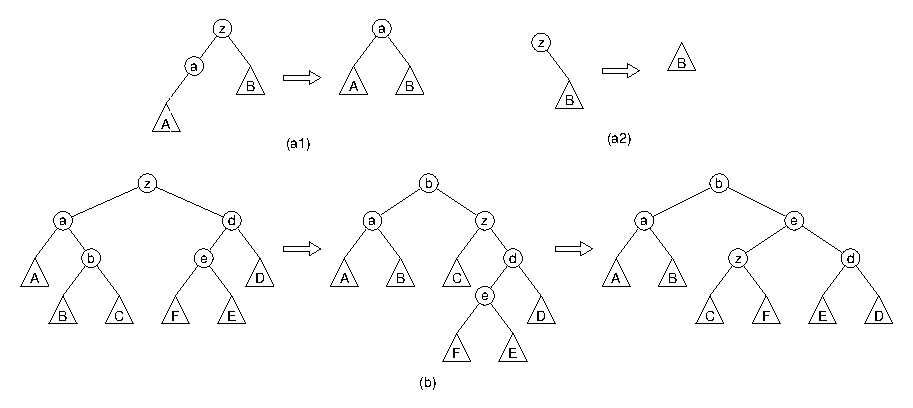
\includegraphics {images/fig4.eps}}
%% \caption{後続操作をブロックしない削除アルゴリズムの1ステップ}
%% \label{figure:delete}
%% \end{figure*}
%% % \end{adjustvboxheight}

%% % \medskip\noindent (b)
%% \item[(b)]
%% ``容易に''削除できない場合:図\ref{figure:delete}(b)のように
%% zig-zagを施し,そ
%% の結果できる$b$の右部分木に,(一つめとは左右対称な) zig-zagを施す.

%% \noindent
%% 4回の回転で$z$は2レベル下降する.$z$の新たな部分木$C$と$F$
%% は,同じレベルにとどまる.それ以外の節点も高々1レベルしか下降
%% しない.$z$を根とする新たな部分木に対して再帰的に削除操作を行なうが,$z$の子孫
%% でない節点がそれによってさらに下降することはない.
%% \end{enumerate}

%% % \medskip
%% 図\ref{figure:zipping}に,根節点$z$の削除による木の形状の変化を示す.
%% \begin{figure*}[t]
%%   \centerline {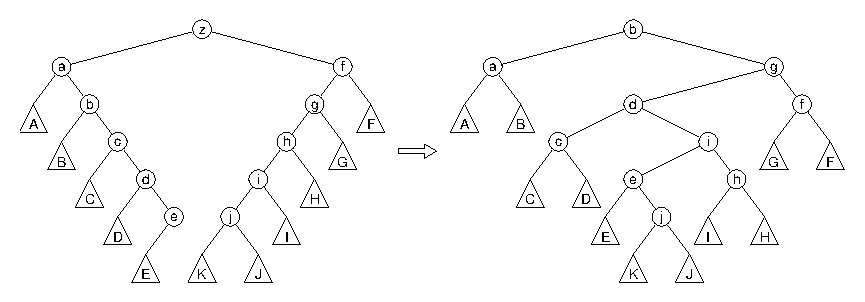
\includegraphics {images/fig5.eps}}
%% \caption{Zippingによる節点$z$の削除}
%% \label{figure:zipping}
%% \end{figure*}

%% 削除対象節点$z$が根であるとは限らない場合は,まず第\ref{section:update}節の
%% 方法で$z$を探索する.これは根から$z$に至るパスを短縮する効果をもつ.つぎ
%% に,$z$をzippingによって下降させて削除する.

%% Zipping操作はパスの短縮を行なわないが,アクセスした節点は浮上させ
%% るという原則にしたがうならば,zippingに先だって,左部分木の最大要素に至
%% るパスと右部分木の最小要素に至るパスをそれぞれトップダウンの半扁平化
%% (zig-zig (図\ref{figure:update}(c)) の繰返し)によっ
%% て短縮すればよい.この短縮化はzippingと並行して行なうことができる.

%% Zippingは更新操作と異なり,各節点のキー値を読むことなく木を下降する.
%% またzippingは,木$T_1$と木$T_2$ ($T_1$のど
%% のキーも,$T_2$のどのキーよりも小さいものとする)とのトップダウン併合操作
%% にも応用できる.すなわち,新たな節点(キーは任意)を調達し,その左部分木
%% を$T_1$,右部分木を$T_2$として一つの木を構成した
%% のち,調達した根節点を消去すればよい.
